%!TEX root = ./HW3.tex

\section{Bandit Problem}
A 10 step and 100 step version of the Bandit Problem were tested.  The same total number of steps was taken, 10,000 steps, but the episode resets occured depnding on the step length of an episode.  The solution quality for the 100 step agent is similar to the 10 step problem.

\subsection{Problem Description}
The goal for the bandit problem is to maximize the expected return given a set of slot machines that give a reward.  In this test, the rewards have a gaussian distrubution and is different for each slot machine.  The number of steps is the number of steps allowed before the situation is reset.  For the Bandit Problem, the initial state is with the accumulated reward as zero.

\subsection{Results}
An action value learning agent is used in both cases.  Figure \ref{fig:Bandit20} and Figure {\ref{fig:Bandit0} shows the expected values as estimated by the learning for both episode lengths with two different exploration amounts along with the actual distribution of the learners.  Table \ref{tab:Bandit} shows statistics of the reward obtained by the agents.

\begin{table}[]
\centering
\begin{tabular}{|c|c|c|c|}
\hline
Steps & Exploration & Reward & StDev \\ \hline
10    & 0.2         & 0.914  & 1.24  \\ \hline
100   & 0.2         & 1.49   & 0.58  \\ \hline
10    & 0.0         & 1.14   & 0.94  \\ \hline
100   & 0.0         & 0.93   & 1.87  \\ \hline
\end{tabular}
\caption{Results for different tests for Bandit Problem with an Action Value learner}
\label{tab:Bandit}
\end{table}

\subsection{Analysis}
All version struggle to approximate the true distribution.  The solutions that they find are within variation of each other indicating that there is no improvement by increasing the length of the episodes. The solution will closer approximate the true distribution as the number of samples increases.  With increased exploration, the true values are generally approximated better.  For action 2 and no exploration, the agent appears to be close to the true value while the many of the other estimates are not close to approximating the true distribution.  

% image of bandit comparison for 20% exploration
\begin{figure}[h]
\centering
\begin{minipage}{0.45\textwidth}
\centering
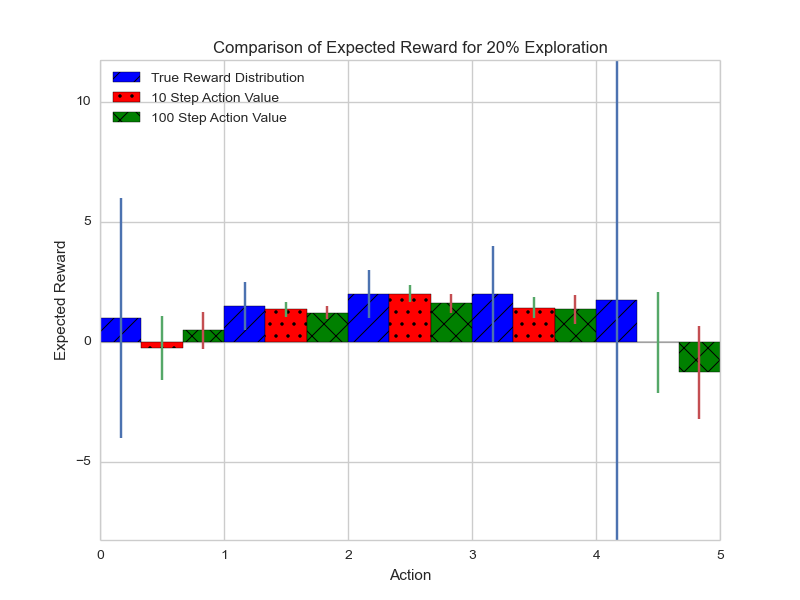
\includegraphics[width=0.98\linewidth]{Bandit20.png}
\caption{Comparison of Action Value tables between selection for 10 steps and 100 steps for an action-value learner with 20\% epsilon greedy exploration  on a multiarmed bandit problem.}
\label{fig:Bandit20}
\end{minipage}%
% image of bandit comparison for 0% exploration
\hspace{0.08\textwidth}%
\begin{minipage}{0.45\textwidth}
\centering
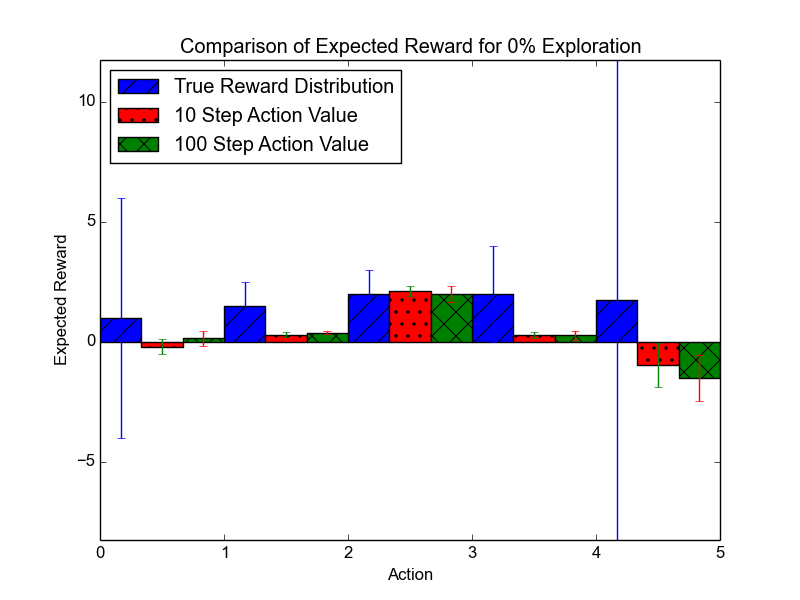
\includegraphics[width=0.98\linewidth]{Bandit0.png}
\caption{Comparison of Action Value tables between selection for 10 steps and 100 steps for an action-value learner with 0\% epsilon greedy exploration  on a multiarmed bandit problem.}
\label{fig:Bandit0}
\end{minipage}
\end{figure}